\documentclass[tikz,border=8pt]{standalone}
\usepackage{amsmath,amssymb}
\usetikzlibrary{arrows.meta,automata,positioning,quotes}
\begin{document}
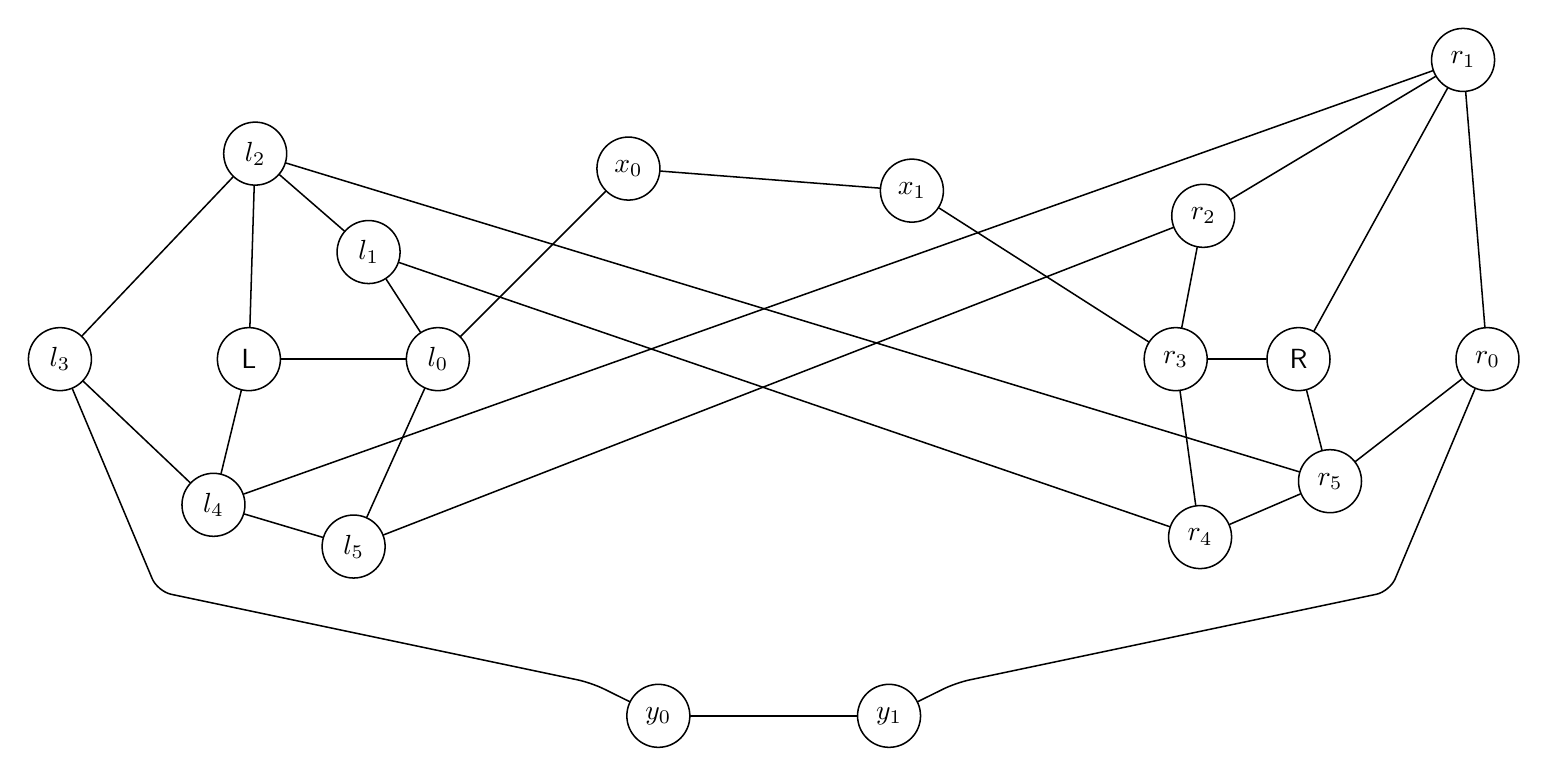
\begin{tikzpicture}[x=1cm,y=1cm]
\tikzset{
  graphnode/.style={circle,draw=black,line width=0.55pt,minimum size=8mm,inner sep=1pt,font=\sffamily},
  graphedge/.style={draw=black,line width=0.55pt,line cap=round,line join=round},
  directed/.style={graphedge,-{Stealth[length=2.4mm,width=2.0mm]}},
  undirected/.style={graphedge}
}
\node[graphnode] (n_L) at (-6.69,0.07) {L};
\node[graphnode] (n_l0) at (-4.29,0.07) {$l_{0}$};
\node[graphnode] (n_l1) at (-5.17,1.43) {$l_{1}$};
\node[graphnode] (n_l2) at (-6.61,2.68) {$l_{2}$};
\node[graphnode] (n_l3) at (-9.09,0.07) {$l_{3}$};
\node[graphnode] (n_l4) at (-7.14,-1.78) {$l_{4}$};
\node[graphnode] (n_l5) at (-5.36,-2.31) {$l_{5}$};
\node[graphnode] (n_R) at (6.64,0.07) {R};
\node[graphnode] (n_r0) at (9.04,0.07) {$r_{0}$};
\node[graphnode] (n_r1) at (8.73,3.87) {$r_{1}$};
\node[graphnode] (n_r2) at (5.43,1.89) {$r_{2}$};
\node[graphnode] (n_r3) at (5.08,0.07) {$r_{3}$};
\node[graphnode] (n_r4) at (5.39,-2.19) {$r_{4}$};
\node[graphnode] (n_r5) at (7.04,-1.48) {$r_{5}$};
\node[graphnode] (n_x0) at (-1.87,2.49) {$x_{0}$};
\node[graphnode] (n_x1) at (1.73,2.21) {$x_{1}$};
\node[graphnode] (n_y0) at (-1.49,-4.46) {$y_{0}$};
\node[graphnode] (n_y1) at (1.44,-4.46) {$y_{1}$};
\draw[undirected] (n_l0) -- (n_l1);
\draw[undirected] (n_l1) -- (n_l2);
\draw[undirected] (n_l2) -- (n_l3);
\draw[undirected] (n_l3) -- (n_l4);
\draw[undirected] (n_l4) -- (n_l5);
\draw[undirected] (n_l5) -- (n_l0);
\draw[undirected] (n_L) -- (n_l0);
\draw[undirected] (n_L) -- (n_l2);
\draw[undirected] (n_L) -- (n_l4);
\draw[undirected] (n_r0) -- (n_r1);
\draw[undirected] (n_r1) -- (n_r2);
\draw[undirected] (n_r2) -- (n_r3);
\draw[undirected] (n_r3) -- (n_r4);
\draw[undirected] (n_r4) -- (n_r5);
\draw[undirected] (n_r5) -- (n_r0);
\draw[undirected] (n_R) -- (n_r1);
\draw[undirected] (n_R) -- (n_r3);
\draw[undirected] (n_R) -- (n_r5);
\draw[undirected] (n_l0) -- (n_x0);
\draw[undirected] (n_x0) -- (n_x1);
\draw[undirected] (n_x1) -- (n_r3);
\draw[undirected,rounded corners=5pt] (n_l3) -- (-7.85,-2.88) -- (-2.34,-4.04) -- (n_y0);
\draw[undirected] (n_y0) -- (n_y1);
\draw[undirected,rounded corners=5pt] (n_r0) -- (7.80,-2.88) -- (2.29,-4.04) -- (n_y1);
\draw[undirected] (n_l1) -- (n_r4);
\draw[undirected] (n_l2) -- (n_r5);
\draw[undirected] (n_l4) -- (n_r1);
\draw[undirected] (n_l5) -- (n_r2);
\end{tikzpicture}
\end{document}
